

\documentclass[a4paper,12pt]{article}

\usepackage{../préambule}
\usepackage{clipboard}

\begin{document}

\Copy{tuiles}{
	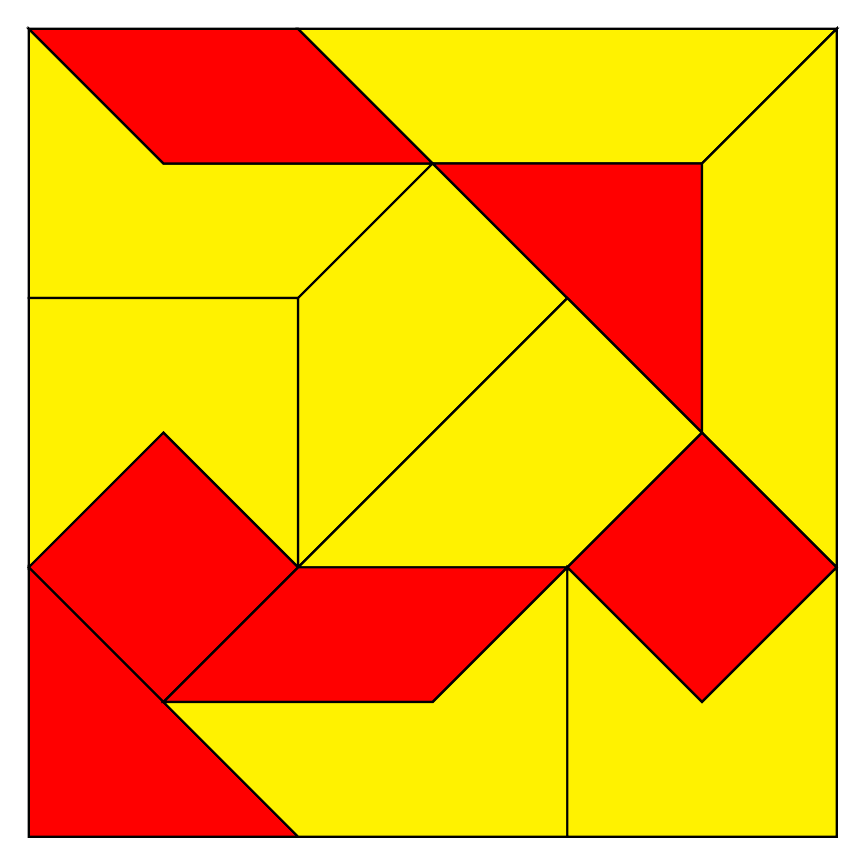
\begin{tikzpicture}[scale=1.71]
		\draw[black,fill=yellow,thick] (0,0) -- ++(0,-2) -- ++(2,0) -- ++(1,1) -- ++(-2,0) -- cycle;
		\draw[black,fill=red,thick] (0,0) -- ++(1,-1) -- ++(2,0) -- ++(-1,1) -- cycle;
		\draw[black,fill=yellow,thick] (2,0) -- ++(1,-1) -- ++(2,0) -- ++(1,1) -- cycle;
		\draw[black,fill=yellow,thick] (3,-1) -- ++(-1,-1) -- ++(0,-2) -- ++(2,2) -- cycle;
		\draw[black,fill=red,thick] (3,-1) -- ++(2,-2) -- ++(0,2) -- cycle;
		\draw[black,fill=yellow,thick] (5,-1) -- ++(0,-2) -- ++(1,-1) -- ++(0,4) -- cycle;
		\draw[black,fill=yellow,thick] (0,-2) -- ++(0,-2) -- ++(1,1) -- ++(1,-1) -- ++(0,2) -- cycle;
		\draw[black,fill=yellow,thick] (2,-4) -- ++(2,0) -- ++(1,1) -- ++(-1,1) -- cycle;
		\draw[black,fill=red,thick] (0,-4) -- ++(1,1) -- ++(1,-1) -- ++(-1,-1) -- cycle;
		\draw[black,fill=red,thick] (0,-4) -- ++(0,-2) -- ++(2,0) -- cycle;

		\draw[black,fill=red,thick] (1,-5) -- ++(2,0) -- ++(1,1) -- ++(-2,0) -- cycle;
		\draw[black,fill=yellow,thick] (1,-5) -- ++(1,-1) -- ++(2,0) -- ++(0,2) -- ++(-1,-1) -- cycle;

		\draw[black,fill=red,thick] (4,-4) -- ++(1,1) -- ++(1,-1) -- ++(-1,-1) -- cycle;
		\draw[black,fill=yellow,thick] (4,-4) -- ++(0,-2) -- ++(2,0) -- ++(0,2) -- ++(-1,-1) -- cycle;
	\end{tikzpicture}
}

\vspace{1.5cm}

\Paste{tuiles}

\end{document}